\begin{figure}[tbp]
\centering
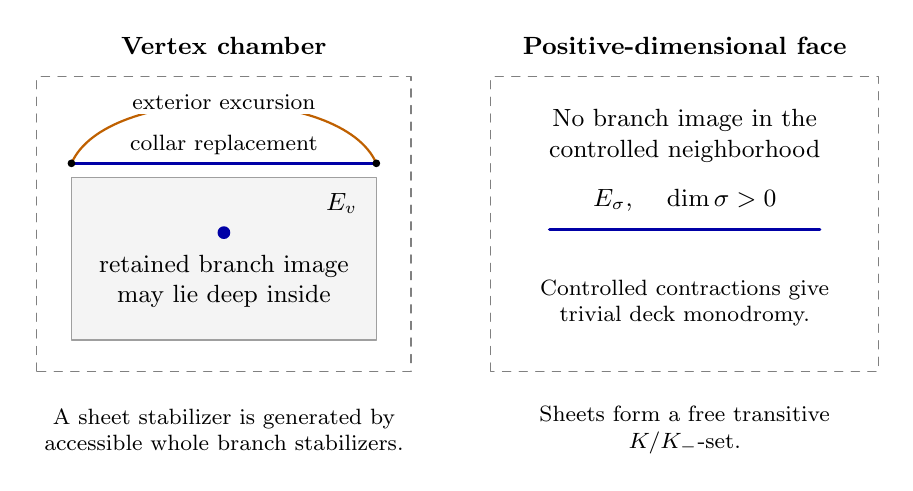
\begin{tikzpicture}[x=.88cm,y=.88cm,font=\small,
  every node/.style={align=center},line cap=round,line join=round]
  \node[font=\small\bfseries] at (2.8,5.35) {Vertex chamber};
  \draw[dashed,gray] (.1,.65) rectangle (5.5,4.9);
  \filldraw[fill=gray!9,draw=gray!75] (.6,1.1) rectangle (5,3.45);
  \node at (4.5,3.07) {$E_v$};
  \fill[blue!65!black] (2.8,2.65) circle (2.3pt);
  \node[text width=3.7cm] at (2.8,1.95)
    {retained branch image\\may lie deep inside};
  \draw[thick,orange!75!black]
    (.6,3.65) .. controls (1.1,4.8) and (4.5,4.8) .. (5,3.65);
  \node[font=\footnotesize,fill=white,inner sep=1.5pt] at (2.8,4.53)
    {exterior excursion};
  \draw[very thick,blue!65!black] (.6,3.65)--(5,3.65);
  \fill (.6,3.65) circle (1.4pt);
  \fill (5,3.65) circle (1.4pt);
  \node[font=\footnotesize,fill=white,inner sep=1pt] at (2.8,3.91)
    {collar replacement};
  \node[font=\footnotesize,text width=4.75cm] at (2.8,-.2)
    {A sheet stabilizer is generated by\\accessible whole branch stabilizers.};

  \node[font=\small\bfseries] at (9.45,5.35)
    {Positive-dimensional face};
  \draw[dashed,gray] (6.65,.65) rectangle (12.25,4.9);
  \node[text width=4.3cm] at (9.45,4.05)
    {No branch image in the\\controlled neighborhood};
  \draw[very thick,blue!65!black] (7.5,2.7)--(11.4,2.7);
  \node at (9.45,3.12) {$E_\sigma$, \quad $\dim\sigma>0$};
  \node[font=\footnotesize,text width=4.35cm] at (9.45,1.63)
    {Controlled contractions give\\trivial deck monodromy.};
  \node[font=\footnotesize,text width=4.85cm] at (9.45,-.2)
    {Sheets form a free transitive\\$K/K_-$-set.};
\end{tikzpicture}
\caption{Schematic coarse neighborhoods for selective cubulation. The
closed mid-halfspace chamber $E_v$ may contain retained branch images;
only the exterior collar used to shorten excursions must avoid them.
Every positive-dimensional face chamber $E_\sigma$ has a branch-free
controlled neighborhood. Consequently sheet transitions between
positive-dimensional faces are equivariant bijections, whereas vertex
sheet stabilizers may be nontrivial. The drawn regions and distances
are schematic: $E_v$ is not asserted to be the literal fiber
$p^{-1}(v)$, and the collar constants do not depend on chamber diameter.}
\label{fig:selective-chambers}
\end{figure}
